\section{A Model for DevOps Adoption}\label{sec:case_study}

Based on H1-H4 hypothesis, in Fig. 2 we present a three step model of how to
adopt DevOps according with our understanding.

\begin{itemize}
\item In the first step, a company should 
disseminate that the goal with a DevOps adoption should be
the establishment of a \cat{collaboration culture} between
development and operations teams.

\item In the second step, a company should select and develop
the most suitable enablers according with its context. The enablers
are means commonly used to develop the \cat{collaboration culture}
and its concepts.

\item In the third step, a company should check the outcomes of the
DevOps adoption in order to verify the alignment with
industrial practices and to explore them according to the
need of the company.
\end{itemize}

\begin{figure*}[H]
  \centering
    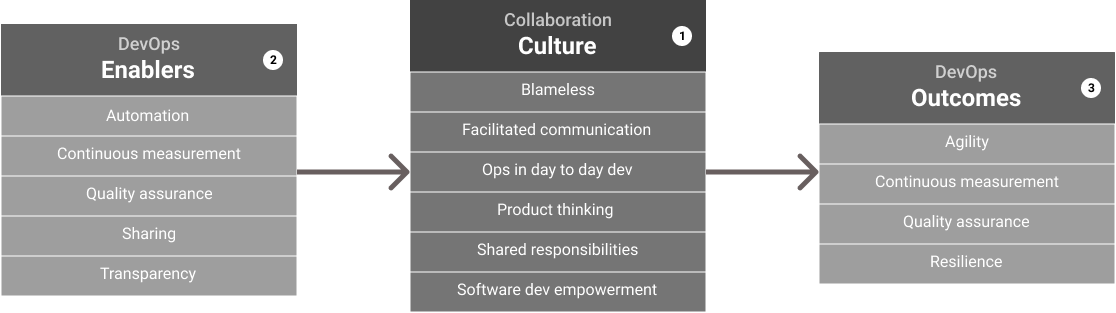
\includegraphics[width=14.26cm,height=4cm,natwidth=1116,natheight=313]{model.png}
    \caption{DevOps Adoption Model}
    \label{fig2}
\end{figure*}


Our proposed model was applied to guide the DevOps adoption in TCU. TCU has the
evolution of DevOps as one of the strategic objectives of its area of
information technology.

{\color{red} Acho que aqui precisa explicar como essas informacoes foram
obtidas, nao sei direito como explicar que um dos autores do artigo trabalha no
TCU}

Before the application of the model, TCU was produced some result in deployment
automation and the focus was being directed to the tooling issue. The conflicts
between development and operations teams continued. The mere advance in
implanting ``DevOps tools" simply changed the points of conflict, but they
persisted.

So, after the presentation of the model in a lecture, development and
operations teams changed their focus to build a collaboration culture. This
change of focus was possible due to the engagement and sponsorship of the IT
managers.

Looking to the concepts in collaboration culture category, the first practical
action in TCU was to facilitate communication between teams. The use of tickets
was abolished. The problems had to be solved in a collaborative way, preferably
face to face. In cases where face to face communication was not feasible, a
communication tool that allowed direct contact could be used.

Looking to enablers, TCU was applied sharing concepts. The role of internal
tech talks and committees to disseminate that collaboration culture and related
concepts was reinforced.

When a new infrastructure had to be provided and configured, the guideline was
that there was a kind of pair programming of developers with infrastructure
analysts. All application related tasks must to be executed in a collaborative
way. Naturally, the professionals noticed that automation would facilitate the
operationalization of that collaboration. So, the infrastructure provisioning
and management was automated. Looking to transparency category, the use of
shared pipelines to contain this automation procedures was set as default.

TCU was also used continuous measurement and quality assurance concepts as
enablers of its DevOps adoption. The applications started to be continuously
tested and measured. The tests were automated and included in the pipelines.
Verifications of test coverage and quality code also were part of the pipeline.
This increased the confidence between teams. With more confidence, TCU started
to explore the potential of DevOps tools, like recovery automation, zero
down-time and auto scaling. The deployment also was automated.

Before DevOps, the deployment historically was a controversial point in TCU.
Several conflicts occurred over time. Rigid procedures were created to try to
avoid problems. There rigid procedures sometimes generated periods of months
without any software delivery.

The collaborative scenario, with strong appeal in automation and quality, created by following an appropriate path in adopting DevOps, enabled the deployment to become a lightweight task in TCU. Continuous deployment became a reality and several deployments occurs in a normal day at software development of TCU.

TCU is a government company. Some advances in DevOps adoption still comes up
against regulatory issues. For example, there are internal regulations that
establish that only the operations sector is responsible for issues related to
application infrastructure, contrasting with shared responsibilities that is
part of collaboration culture.

The model enabled TCU to adopt DevOps in a more sustainable way. Know the role
of each DevOps element in the adoption was fundamental for TCU to avoid points
of failure and to build a collaborative environment that supports the
exploitation of DevOps benefits in the long run.
